% topic2.tex -- Topic 2: Circular motion and torque, Questions 25-48.
\topictitle{Topic 2 - Circular Motion}

% ---- Q25 (string breaks: tangent path)
\begin{quizq}{}
A puck on a string moves anticlockwise in a horizontal circle around a central point, $O$, on a flat,
frictionless table. The diagram shows the view from above.
\begin{center}
  \begin{tikzpicture}
    \draw[guide] (0,0) circle (1.6);
    \draw[line width=1.6pt] (0,0) -- (0,-1.6); \fill (0,0) circle (1.5pt) node[above left, font=\small] {$O$};
    \node[left, font=\small] at (0,-0.8) {String};
    \draw[->, line width=0.7pt] (-1.6,0.25) -- (-1.6,-0.25);
    \node[left, font=\small, align=right] at (-1.65,0) {Direction\\of motion};
    \draw[line width=0.8pt, domain=0:40, samples=20, smooth] plot ({1.6*sin(\x)}, {-1.6*cos(\x)});
    \node[above right, font=\small] at ({1.6*sin(40)}, {-1.6*cos(40)}) {$A$};
    \draw[line width=0.8pt] (0,-1.6) -- (1.9,-1.6) node[right, font=\small] {$B$};
    \draw[line width=0.8pt, domain=0:1.7, samples=20, smooth] plot (\x, {-1.6-0.3*\x*\x});
    \node[right, font=\small] at (1.7,-2.47) {$C$};
    \draw[line width=0.8pt] (0,-1.6) -- (0,-2.7) node[below, font=\small] {$D$};
    \fill (0,-1.6) circle (3pt); \node[below left, font=\small] at (0,-1.6) {$X$};
  \end{tikzpicture}
\end{center}
The string breaks as the puck passes point $X$. Which line best shows the path of the puck after
this?
\opts{Line $A$}{Line $B$}{Line $C$}{Line $D$}
\end{quizq}

% ---- Q26 (force needed for a given torque)
\Needspace{12\baselineskip}
\begin{quizq}{}
A wheel nut must be tightened with a torque of \qty{90}{N.m}. The wrench is \qty{0.40}{m} long. The
force is applied at the end of the wrench, at \ang{60} to the wrench.

How much force must be applied?
\opts{\qty{31}{N}}{\qty{225}{N}}{\qty{260}{N}}{\qty{450}{N}}
\end{quizq}

% ---- Q27 (doubling the torque on a door)
\Needspace{15\baselineskip}
\begin{quizq}{}
A person pushes on a door at \ang{90} to the door, at the handle. Which change would \emph{double}
the torque about the hinges?
\opts{Pushing at the same point with the same force, but at \ang{30} to the door}
  {Pushing halfway between the handle and the hinges with twice the force, at \ang{90} to the door}
  {Pushing at the hinges with four times the force}
  {Pushing at the same point with twice the force, at \ang{90} to the door}
\end{quizq}

% ---- Q28 (largest torque on a bar)
% Torques: A = FL, B = 2F x L/2 = FL, C = 3F x L x sin 30 = 1.5 FL, D = 0 (along the bar).
\Needspace{30\baselineskip}
\begin{quizq}{}
A light bar can turn about a pivot at its left end. Forces are applied to the bar as shown.

In which diagram is the torque about the pivot the largest?
\gridopts{%
  \begin{tikzpicture}[scale=1.15]
    \path (-0.4,-0.8) rectangle (4.3,1.4);
    \draw[fill=black!15] (0,-0.08) rectangle (3,0.08); \fill (0,0) circle (2.5pt);
    \draw[force] (3,0.08) -- (3,0.9) node[right] {$F$};
    \draw[|<->|, line width=0.4pt] (0,-0.4) -- (3,-0.4) node[midway, below, font=\small] {$L$};
  \end{tikzpicture}}
  {%
  \begin{tikzpicture}[scale=1.15]
    \path (-0.4,-0.8) rectangle (4.3,1.4);
    \draw[fill=black!15] (0,-0.08) rectangle (3,0.08); \fill (0,0) circle (2.5pt);
    \draw[force] (1.5,0.08) -- (1.5,1.3) node[right] {$2F$};
    \draw[|<->|, line width=0.4pt] (0,-0.4) -- (1.5,-0.4) node[midway, below, font=\small] {$L/2$};
  \end{tikzpicture}}
  {%
  \begin{tikzpicture}[scale=1.15]
    \path (-0.4,-0.8) rectangle (4.3,1.4);
    \draw[fill=black!15] (0,-0.08) rectangle (3,0.08); \fill (0,0) circle (2.5pt);
    \draw[force] (3,0) -- ({3+1.25*cos(30)},{1.25*sin(30)}) node[above] {$3F$};
    \draw[guide] (3,0) -- (4.2,0);
    \draw (3.6,0) arc (0:30:0.6); \node[font=\scriptsize] at (3.85,0.18) {\ang{30}};
    \draw[|<->|, line width=0.4pt] (0,-0.4) -- (3,-0.4) node[midway, below, font=\small] {$L$};
  \end{tikzpicture}}
  {%
  \begin{tikzpicture}[scale=1.15]
    \path (-0.4,-0.8) rectangle (4.3,1.4);
    \draw[fill=black!15] (0,-0.08) rectangle (3,0.08); \fill (0,0) circle (2.5pt);
    \draw[force] (3,0) -- (4.1,0) node[above] {$4F$};
    \draw[|<->|, line width=0.4pt] (0,-0.4) -- (3,-0.4) node[midway, below, font=\small] {$L$};
  \end{tikzpicture}}
\end{quizq}

% ---- Q29 (time to move through an angle)
\Needspace{24\baselineskip}
\begin{quizq}{}
A toy car moves clockwise at a constant speed around a circular track. It completes 5 laps in
\qty{8.0}{s}.
\begin{center}
  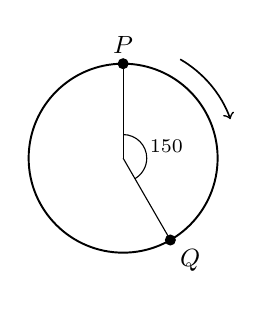
\begin{tikzpicture}
    \draw[line width=0.7pt] (0,0) circle (1.2);
    \draw (0,0) -- (0,1.2); \draw (0,0) -- ({1.2*cos(-60)},{1.2*sin(-60)});
    \fill (0,1.2) circle (2pt) node[above, font=\small] {$P$};
    \fill ({1.2*cos(-60)},{1.2*sin(-60)}) circle (2pt) node[below right, font=\small] {$Q$};
    \draw (0,0.3) arc (90:-60:0.3); \node[font=\scriptsize] at (0.55,0.15) {\ang{150}};
    \draw[->, line width=0.6pt] (60:1.45) arc (60:20:1.45);
  \end{tikzpicture}
\end{center}
How long does the car take to move from point $P$ to point $Q$?
\opts{\qty{0.67}{s}}{\qty{0.93}{s}}{\qty{3.3}{s}}{\qty{38}{s}}
\end{quizq}

% ---- Q30 (centripetal force from frequency)
\Needspace{12\baselineskip}
\begin{quizq}{}
A \qty{150}{g} rubber stopper is whirled on a string in a horizontal circle of radius \qty{0.80}{m}.
It makes 2.0 revolutions every second.

What is the centripetal force on the stopper?
\opts{\qty{0.48}{N}}{\qty{1.2}{N}}{\qty{19}{N}}{\qty{1.9e4}{N}}
\end{quizq}

% ---- Q31 (banked track above the design speed)
\Needspace{15\baselineskip}
\begin{quizq}{}
A car goes around a banked curve at a constant speed that is \emph{greater} than the design speed of
the curve. The car does not slide.

Compared with travelling at the design speed, which extra force acts on the car to help provide the
larger centripetal force?
\opts{A friction force acting up the slope}{A friction force acting down the slope}
  {A larger weight force}{An outward centrifugal force}
\end{quizq}

% ---- Q32 (acceleration when v is halved and r is tripled)
\Needspace{12\baselineskip}
\begin{quizq}{}
An object moves in a circle of radius $r$ at a constant speed $v$. Its centripetal acceleration is
$a$. The speed is halved and the radius is tripled.

What is the new centripetal acceleration?
\opts{$\dfrac{a}{12}$}{$\dfrac{a}{6}$}{$\dfrac{3a}{4}$}{$\dfrac{4a}{3}$}
\end{quizq}

% ---- Q33 (direction of the net force on a banked track)
\Needspace{26\baselineskip}
\begin{quizq}{}
A vehicle moves around a horizontal circular track which is banked, as shown. The centre of the
circle is to the left. The vehicle's speed is constant and it stays at the same height on the
track.
\begin{center}
  \begin{tikzpicture}[scale=1.25]
    \draw[line width=0.6pt] (-0.6,0) -- (5.6,0);
    \draw[line width=0.8pt] (0,0) -- (5.2,{5.2*tan(25)});
    \draw ({0.9},0) arc (0:25:0.9); \node[font=\scriptsize] at (1.15,0.2) {$\theta$};
    \begin{scope}[shift={({3.2*cos(25)},{3.2*sin(25)})}, rotate=25]
      \draw[fill=black!8, rounded corners=2pt] (-0.65,0.12) rectangle (0.65,0.75);
      \draw[fill=white] (-0.4,0.12) circle (0.12); \draw[fill=white] (0.4,0.12) circle (0.12);
    \end{scope}
    \coordinate (C) at (2.75,1.75);
    \draw[force] (C) -- ++({-1.3*sin(25)},{1.3*cos(25)}) node[above, font=\small\bfseries] {A};
    \draw[force] (C) -- ++({-1.4*cos(25)},{-1.4*sin(25)}) node[left, font=\small\bfseries] {B};
    \draw[force] (C) -- ++(-1.5,0) node[left, font=\small\bfseries] {C};
    \draw[force] (C) -- ++(0,-1.3) node[below, font=\small\bfseries] {D};
  \end{tikzpicture}
\end{center}
Which arrow correctly represents the direction of the net force acting on the vehicle?
\opts{$A$}{$B$}{$C$}{$D$}
\end{quizq}

% ---- Q34 (torque on a disc, force at an angle)
\Needspace{26\baselineskip}
\begin{quizq}{}
A disc of radius \qty{0.50}{m} can rotate about an axis through its centre. A \qty{40}{N} force is
applied at the edge of the disc, at \ang{25} to the line of the radius, as shown.
\begin{center}
  \begin{tikzpicture}
    \draw[fill=black!8, line width=0.7pt] (0,0) circle (1.5);
    \fill (0,0) circle (2pt) node[below, font=\small] {Axis};
    \draw[->, line width=0.8pt] (0,0) -- ({1.5*cos(30)},{1.5*sin(30)}) node[midway, above left, font=\small] {\qty{0.50}{m}};
    \draw[guide] ({1.5*cos(30)},{1.5*sin(30)}) -- ({2.8*cos(30)},{2.8*sin(30)});
    \draw[force] ({1.5*cos(30)},{1.5*sin(30)}) -- ++({1.3*cos(55)},{1.3*sin(55)}) node[above, font=\small] {\qty{40}{N}};
    \draw ({1.5*cos(30)+0.55*cos(30)},{1.5*sin(30)+0.55*sin(30)}) arc (30:55:0.55);
    \node[font=\scriptsize] at ({1.5*cos(30)+0.8*cos(42)},{1.5*sin(30)+0.8*sin(42)}) {\ang{25}};
  \end{tikzpicture}
\end{center}
What is the size of the torque about the axis?
\opts{\qty{8.5}{N.m}}{\qty{18}{N.m}}{\qty{20}{N.m}}{\qty{845}{N.m}}
\end{quizq}

% ---- Q35 (speed from the hanging mass)
\Needspace{28\baselineskip}
\begin{quizq}{}
A hanging mass $M$ is used to keep a rubber stopper of mass $m$ in uniform circular motion of radius
$r$, as shown. The stopper moves at speed $v$.
\begin{center}
  \begin{tikzpicture}
    \draw[guide] (0,2.6) ellipse (1.8 and 0.35);
    \draw[fill=black!8] (-0.08,0.9) rectangle (0.08,2.6);
    \draw[line width=0.7pt] (0,2.6) -- (1.75,2.6); \draw[fill=black!40] (1.75,2.48) rectangle (1.98,2.72);
    \draw[line width=0.7pt] (0,0.9) -- (0,0.55); \draw[fill=black!40] (-0.18,0.2) rectangle (0.18,0.55);
    \node[right, font=\small] at (2.0,2.6) {Rubber stopper ($m$)};
    \node[right, font=\small] at (0.25,0.38) {Hanging mass ($M$)};
    \node[right, font=\small] at (0.15,1.6) {Glass tube};
    \node[above, font=\small] at (0.9,2.6) {$r$};
  \end{tikzpicture}
\end{center}
Assuming all friction is negligible, which expression gives the speed $v$ of the stopper?
\opts{$\sqrt{\dfrac{mgr}{M}}$}{$\dfrac{Mgr}{m}$}{$\sqrt{\dfrac{Mg}{mr}}$}{$\sqrt{\dfrac{Mgr}{m}}$}
\end{quizq}

% ---- Q36 (mass from force, angular velocity and radius)
\Needspace{13\baselineskip}
\begin{quizq}{}
A ball on a string is swung in a horizontal circle of radius \qty{60}{cm}. A force meter shows that
the centripetal force on the ball is \qty{3.2}{N}. The angular velocity is $3\pi$~\si{rad.s^{-1}}.

What is the mass of the ball?
\opts{\qty{0.022}{kg}}{\qty{0.060}{kg}}{\qty{0.57}{kg}}{\qty{0.59}{kg}}
\end{quizq}

% ---- Q37 (projectile motion compared with circular motion)
\Needspace{18\baselineskip}
\begin{quizq}{}
Which statement best describes a difference between projectile motion and uniform circular motion?
\opts{In projectile motion, the net force is constant in size and direction. In uniform circular
   motion, the net force is constant in size but always changes direction.}
  {In projectile motion, the acceleration is zero at the highest point. In uniform circular
   motion, the acceleration is never zero.}
  {In projectile motion, the speed is constant. In uniform circular motion, the speed changes.}
  {In projectile motion, the net force does no work. In uniform circular motion, the net force does
   work.}
\end{quizq}

% ---- Q38 (banking angle)
\Needspace{12\baselineskip}
\begin{quizq}{}
A curve on a highway has a radius of \qty{120}{m}. It is banked so that cars travelling at
\qty{72}{km.h^{-1}} need no friction to go around it.

To the nearest degree, at what angle is the road banked?
\opts{\ang{1}}{\ang{19}}{\ang{71}}{\ang{77}}
\end{quizq}

% ---- Q39 (which graph is linear: F against 1/T^2)
\Needspace{15\baselineskip}
\begin{quizq}{}
In an investigation, a student whirls a rubber stopper in a horizontal circle of fixed radius. A
hanging mass provides the centripetal force $F$. The student changes $F$ and measures the period
$T$ each time.

Which graph should give a straight line through the origin?
\opts{$F$ (vertical axis) against $T$ (horizontal axis)}
  {$F$ (vertical axis) against $T^2$ (horizontal axis)}
  {$F$ (vertical axis) against $\dfrac{1}{T}$ (horizontal axis)}
  {$F$ (vertical axis) against $\dfrac{1}{T^2}$ (horizontal axis)}
\end{quizq}

% ---- Q40 (sideways accelerometer on a winding road)
\Needspace{46\baselineskip}
\begin{quizq}{}
A car travels at a constant speed along the road shown (view from above). It drives straight, turns
left, drives straight, then turns right.
\begin{center}
  \begin{tikzpicture}[scale=1.1]
    \draw[guide, line width=0.8pt] (0,0) -- (0,1) arc (0:90:1) -- (-2,2) arc (270:180:1) -- (-3,4);
    \draw[->, line width=0.7pt] (0.25,-0.1) -- (0.25,0.6);
    \node[right, font=\small] at (0.1,0) {Start};
    \node[left, font=\small] at (-3,4) {Finish};
    \node[right, font=\scriptsize] at (0.05,1.75) {turn left}; \node[left, font=\scriptsize] at (-2.75,2.45) {turn right};
  \end{tikzpicture}
\end{center}
An accelerometer fixed in the car measures the sideways acceleration of the car. Acceleration
towards the car's \emph{left} side is positive.

Which graph shows the measurements recorded by the accelerometer?
\gridopts{%
  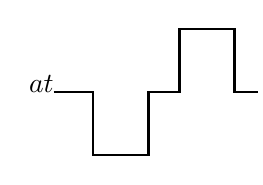
\begin{tikzpicture}\gaxesPN{$a$}{$t$}
    \draw[line width=1pt] (0,0) -- (0.5,0) -- (0.5,-0.8) -- (1.2,-0.8) -- (1.2,0) -- (1.6,0) -- (1.6,0.8) -- (2.3,0.8) -- (2.3,0) -- (2.6,0);
  \end{tikzpicture}}
  {%
  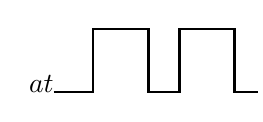
\begin{tikzpicture}\gaxesPN{$a$}{$t$}
    \draw[line width=1pt] (0,0) -- (0.5,0) -- (0.5,0.8) -- (1.2,0.8) -- (1.2,0) -- (1.6,0) -- (1.6,0.8) -- (2.3,0.8) -- (2.3,0) -- (2.6,0);
  \end{tikzpicture}}
  {%
  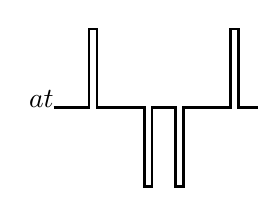
\begin{tikzpicture}\gaxesPN{$a$}{$t$}
    \draw[line width=1pt] (0,0) -- (0.45,0) -- (0.45,1.0) -- (0.55,1.0) -- (0.55,0) -- (1.15,0) -- (1.15,-1.0) -- (1.25,-1.0) -- (1.25,0) -- (1.55,0) -- (1.55,-1.0) -- (1.65,-1.0) -- (1.65,0) -- (2.25,0) -- (2.25,1.0) -- (2.35,1.0) -- (2.35,0) -- (2.6,0);
  \end{tikzpicture}}
  {%
  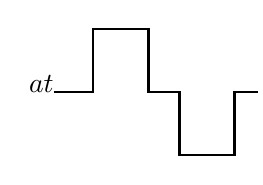
\begin{tikzpicture}\gaxesPN{$a$}{$t$}
    \draw[line width=1pt] (0,0) -- (0.5,0) -- (0.5,0.8) -- (1.2,0.8) -- (1.2,0) -- (1.6,0) -- (1.6,-0.8) -- (2.3,-0.8) -- (2.3,0) -- (2.6,0);
  \end{tikzpicture}}
\end{quizq}

% ---- Q41 (conical pendulum)
\Needspace{26\baselineskip}
\begin{quizq}{}
A tether ball moves in uniform circular motion in a horizontal circle of radius $r$ around a pole.
The string makes an angle $\theta$ with the vertical pole.
\begin{center}
  \begin{tikzpicture}
    \fill[black!25] (-0.07,0) rectangle (0.07,3.4);
    \draw[guide] (0,1.2) ellipse (1.3 and 0.3);
    \draw[line width=0.7pt] (0,3.2) -- (1.3,1.2);
    \draw (0,2.7) arc (270:303:0.5); \node[font=\scriptsize] at (0.18,2.45) {$\theta$};
    \draw[|<->|, line width=0.4pt] (0,1.2) -- (1.3,1.2) node[midway, below, font=\small] {$r$};
    \shade[ball color=black!20] (1.3,1.2) circle (0.15);
  \end{tikzpicture}
\end{center}
Which expression gives the speed $v$ of the ball?
\opts{$\sqrt{rg\tan\theta}$}{$\sqrt{\dfrac{rg}{\tan\theta}}$}{$\sqrt{rg\sin\theta}$}{$rg\tan\theta$}
\end{quizq}

% ---- Q42 (tension in a vertical circle at constant speed)
% Correct: T = mv^2/r - mg cos(angle from top): smallest at the top, largest at the bottom.
\Needspace{40\baselineskip}
\begin{quizq}{}
A ball on a string moves in a vertical circle at a constant speed, as shown. It starts at the top of
the circle.
\begin{center}
  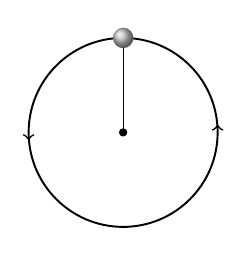
\begin{tikzpicture}
    \draw[line width=0.7pt] (0,0) circle (1.2);
    \draw (0,0) -- (0,1.2); \fill (0,0) circle (1.5pt);
    \shade[ball color=black!25] (0,1.2) circle (0.13);
    \draw[->, line width=0.6pt] (-1.2,0.1) -- (-1.2,-0.1);
    \draw[->, line width=0.6pt] (1.2,-0.1) -- (1.2,0.1);
  \end{tikzpicture}
\end{center}
Which graph correctly shows the tension in the string as the ball completes one revolution from the
top?
\gridopts{%
  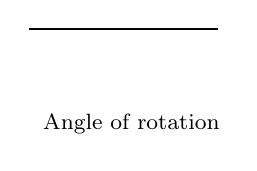
\begin{tikzpicture}\gaxesP{Tension}{}
    \draw[line width=1pt] (0,0.9) -- (2.4,0.9);
    \node[below, font=\footnotesize] at (1.3,-0.05) {Angle of rotation};
  \end{tikzpicture}}
  {%
  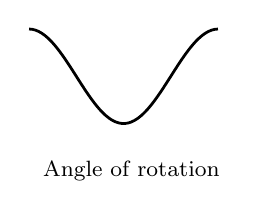
\begin{tikzpicture}\gaxesP{Tension}{}
    \draw[line width=1pt, domain=0:2.4, samples=60, smooth] plot (\x, {0.9 + 0.6*cos(150*\x)});
    \node[below, font=\footnotesize] at (1.3,-0.05) {Angle of rotation};
  \end{tikzpicture}}
  {%
  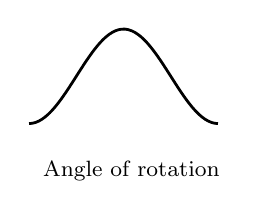
\begin{tikzpicture}\gaxesP{Tension}{}
    \draw[line width=1pt, domain=0:2.4, samples=60, smooth] plot (\x, {0.9 - 0.6*cos(150*\x)});
    \node[below, font=\footnotesize] at (1.3,-0.05) {Angle of rotation};
  \end{tikzpicture}}
  {%
  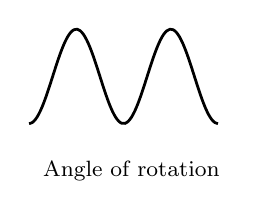
\begin{tikzpicture}\gaxesP{Tension}{}
    \draw[line width=1pt, domain=0:2.4, samples=60, smooth] plot (\x, {0.9 - 0.6*cos(300*\x)});
    \node[below, font=\footnotesize] at (1.3,-0.05) {Angle of rotation};
  \end{tikzpicture}}
\end{quizq}

% ---- Q43 (puck inside a smooth circular wall)
\Needspace{16\baselineskip}
\begin{quizq}{}
A puck slides at a constant speed around the inside of a smooth, circular, vertical wall. It moves
on a flat, horizontal, frictionless table, touching the wall all the time.

Which statement correctly describes the net force acting on the puck?
\opts{The net force is zero, because the speed is constant.}
  {The net force acts in the direction of motion of the puck.}
  {The net force acts away from the centre of the circle, because of the centrifugal force.}
  {The net force acts towards the centre of the circle. It is provided by the normal force from the
   wall.}
\end{quizq}

% ---- Q44 (minimum speed at the top of a vertical loop)
\Needspace{24\baselineskip}
\begin{quizq}{}
A roller-coaster car travels around a vertical circular loop of radius \qty{8.0}{m}.
\begin{center}
  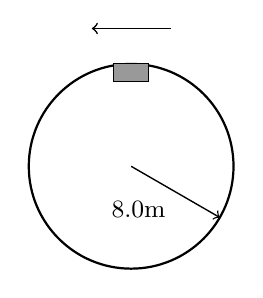
\begin{tikzpicture}
    \draw[line width=0.8pt] (0,0) circle (1.3);
    \draw[->, line width=0.5pt] (0,0) -- (-30:1.3) node[midway, below left, font=\small] {\qty{8.0}{m}};
    \draw[fill=black!40] (-0.22,1.08) rectangle (0.22,1.3);
    \draw[->, line width=0.6pt] (0.5,1.75) -- (-0.5,1.75);
  \end{tikzpicture}
\end{center}
What is the minimum speed, in \si{m.s^{-1}}, at which the car must travel at the top of the loop
to stay on the circular path?
\opts{1.1}{8.9}{12.5}{78}
\end{quizq}

% ---- Q45 (maximum speed on a flat bend)
\Needspace{12\baselineskip}
\begin{quizq}{}
A \qty{1200}{kg} car goes around a flat, horizontal bend of radius \qty{50}{m}. The maximum
sideways friction force the road can provide is \qty{9600}{N}.

What is the maximum speed at which the car can go around the bend without sliding?
\opts{\qty{0.40}{m.s^{-1}}}{\qty{8.0}{m.s^{-1}}}{\qty{20}{m.s^{-1}}}{\qty{400}{m.s^{-1}}}
\end{quizq}

% ---- Q46 (speed of a point on a rotating wheel)
\Needspace{11\baselineskip}
\begin{quizq}{}
A wheel of radius \qty{0.30}{m} rotates at 120 revolutions per minute. What is the speed of a point
on the rim of the wheel?
\opts{\qty{0.60}{m.s^{-1}}}{\qty{3.8}{m.s^{-1}}}{\qty{36}{m.s^{-1}}}{\qty{226}{m.s^{-1}}}
\end{quizq}

% ---- Q47 (work done by the centripetal force)
\Needspace{12\baselineskip}
\begin{quizq}{}
A \qty{0.50}{kg} mass on a string moves in a horizontal circle of radius \qty{1.2}{m} at a constant
speed of \qty{4.0}{m.s^{-1}} on a frictionless table.

How much work does the tension in the string do on the mass during one revolution?
\opts{\qty{0}{J}}{\qty{4.0}{J}}{\qty{8.0}{J}}{\qty{50}{J}}
\end{quizq}

% ---- Q48 (crank position for the largest torque)
\Needspace{15\baselineskip}
\begin{quizq}{}
A cyclist pushes straight down on a pedal with a constant force as the crank turns. At which crank
position is the torque about the axle the greatest?
\opts{When the crank points vertically upwards}{When the crank points \ang{45} below the horizontal}
  {When the crank points vertically downwards}{When the crank is horizontal}
\end{quizq}
